\documentclass{article}
\usepackage{amsmath}
\usepackage{amsthm}
\usepackage{amsfonts}
\usepackage{amssymb}
\usepackage{bbold}
\usepackage{dsfont}
\usepackage{graphicx}
\usepackage{cleveref}
\usepackage{bm}
\usepackage{booktabs}
\usepackage{siunitx}
\usepackage{xcolor}
\usepackage[utf8]{inputenc}
\usepackage[english]{babel}
\newtheorem{definition}{Definition}
\newtheorem{example}{Example}
\newcommand{\exP}[1]{\mathrm{e}^{#1}}
\newcommand{\dif}{\mathrm{d}}
\renewcommand{\vec}[1]{\mathbf{#1}}
\newcommand{\pdagger}{{\phantom{\dagger}}}
\newcommand{\state}[1]{\vert #1\rangle}
\newcommand{\cstate}[1]{\langle #1\vert}
\newcommand{\tr}[1]{\mathrm{tr}\left\{#1\right\}}
\newcommand{\trs}[2]{\, \mathrm{tr}_{#1}\{#2\}}
\newcommand{\expc}[3]{\langle #1\vert #2 \vert #3\rangle}
\usepackage[doi=false,url=false,isbn=false,backend=bibtex,style=nature,natbib=true,sorting=none]{biblatex}
\bibliography{bib.bib}
\usepackage{geometry}
\geometry{
	a4paper,
	total={170mm,257mm},
	left=20mm,
	top=20mm,
}
\begin{document}
\title{Report 6: Investigation of spin-less Peierls and spin-full Fransson models for varying system sizes within TTHEOM approach}
\author{Rudolf Smorka}
\maketitle
\section{Spin-less charge transport through one-dimensional Peierls chains}
\subsection{Model}
The system is modeled by the spin-less Peierls-model, that is a collection of $N$ sites and $N-1$ vibrational modes 
\begin{equation}
	H_\mathrm{sys} = \sum_j^N \varepsilon_j^\pdagger d_j^\dagger d_j^\pdagger + \sum_j^N \omega_j^\pdagger a_j^\dagger a_j^\pdagger - \sum_j (t_0+t_1(a_j^\dagger + a_j^\pdagger))(d_{j}^\dagger d_{j+1}^\pdagger + \mathrm{h.c.}).
\end{equation}
The bond between sites $j$ and $j+1$ is described by a single harmonic mode with frequency $\omega_j$.
In the following, the on-site energies are set to $\varepsilon_j = \SI{-240}{\milli\electronvolt}$, the vibrational frequencies are $\omega_j = \SI{2}{\milli\electronvolt}$, the hopping matrix element is $t_0 = \SI{40}{\milli\electronvolt}$ and the Peierls-coupling is $t_1 = \SI{4}{\milli\electronvolt}$. This system is attached to two fermionic leads, modeled by 
\begin{equation}
	H_\mathrm{leads} = \sum_{\ell=L,R}\sum_k \varepsilon_{\ell k}^\pdagger c_{\ell k}^\dagger  c_{\ell k}^\pdagger.
\end{equation}
The first site of the system is coupled to the left lead and the last site of the system is coupled to the right lead, whereas the coupling is linear in the system and environment degrees of freedom
\begin{equation}
	H_\mathrm{sys-lead} = \sum_{\ell k} (V_{\ell k 1}^\pdagger c_{\ell k}^\dagger d_1^\pdagger + V_{\ell k N}^\pdagger c_{\ell k}^\dagger d_N^\pdagger + \mathrm{h.c.}).
\end{equation}
The system-lead coupling is characterized by the spectral function 
\begin{equation}
	\Gamma_i^{(\ell)}(\varepsilon) = 2\pi \sum_k \vert V_{\ell k i}\vert^2 \delta(\varepsilon_i-\varepsilon_{\ell k}),
\end{equation}
which we take as constant with value $\Gamma^{(\ell)}= \SI{10}{\milli\electronvolt}$ for both leads. Also, both leads are held at room temperature $T=\SI{25}{\milli\electronvolt}$.
\clearpage
\subsection{$N = 3$}
\begin{figure}[!h]
	\centering
	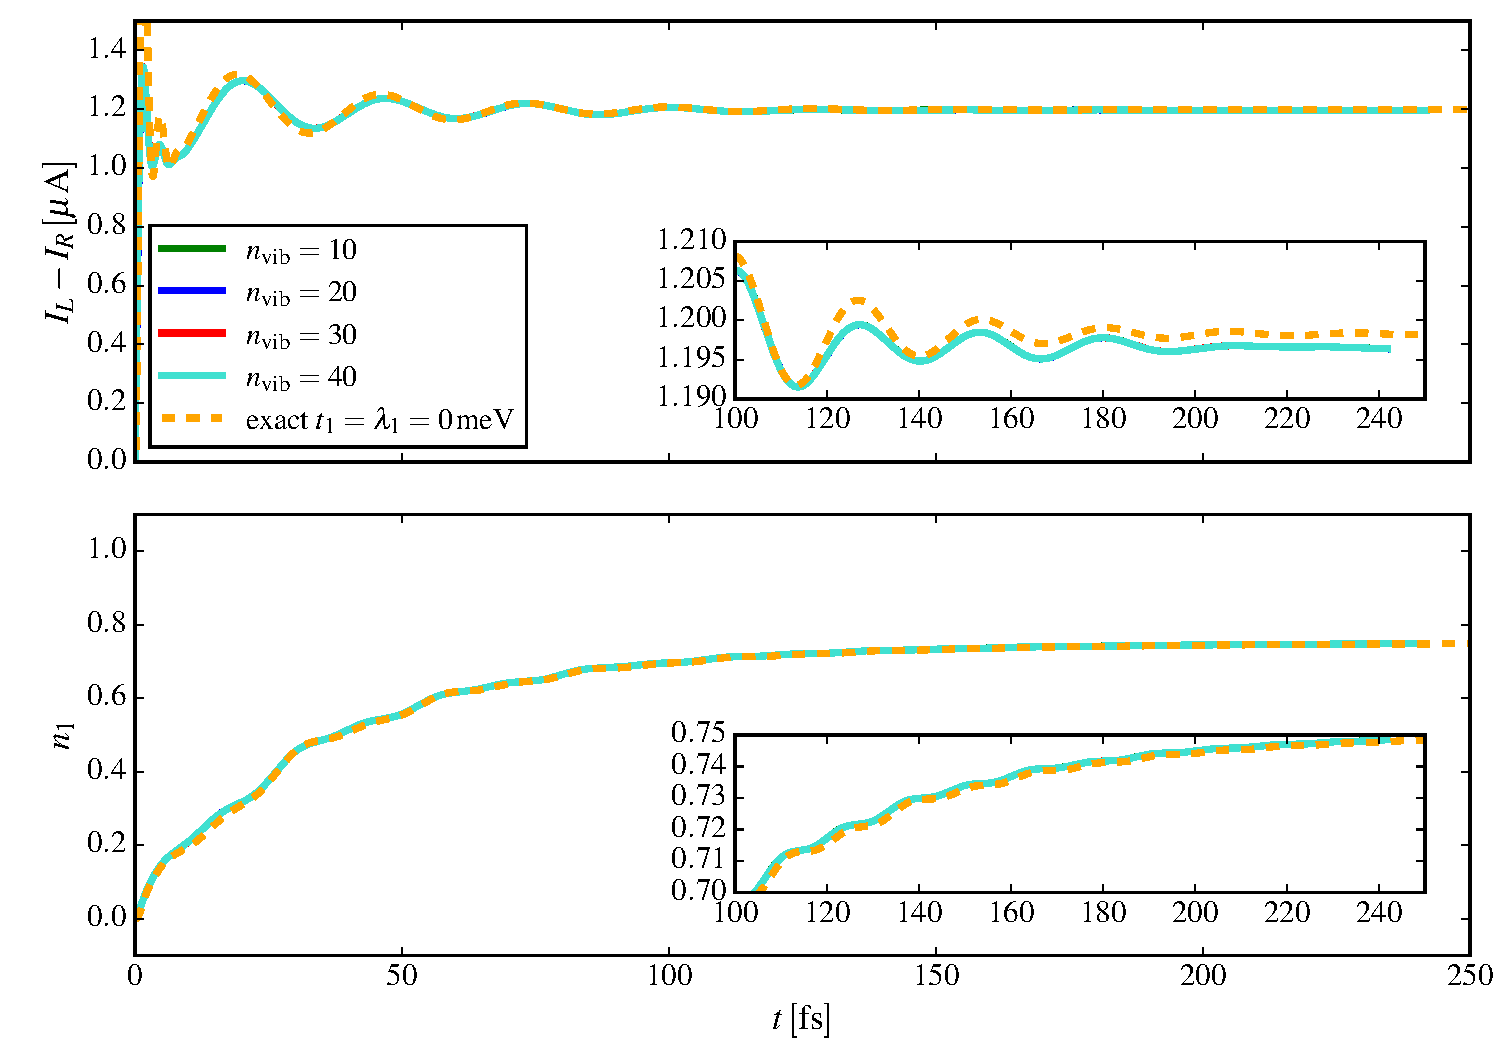
\includegraphics[width=0.85\textwidth]{figs/Comparison_TTHEOM_MFHEOM_Holstein_1x3_noSpin_w0_0.05_V0.48.pdf}
	\caption{Symmetrized current and electronic population on site 1 for $N=3$.}
\end{figure}
\subsection{$N = 4$}
\begin{figure}[!h]
	\centering
	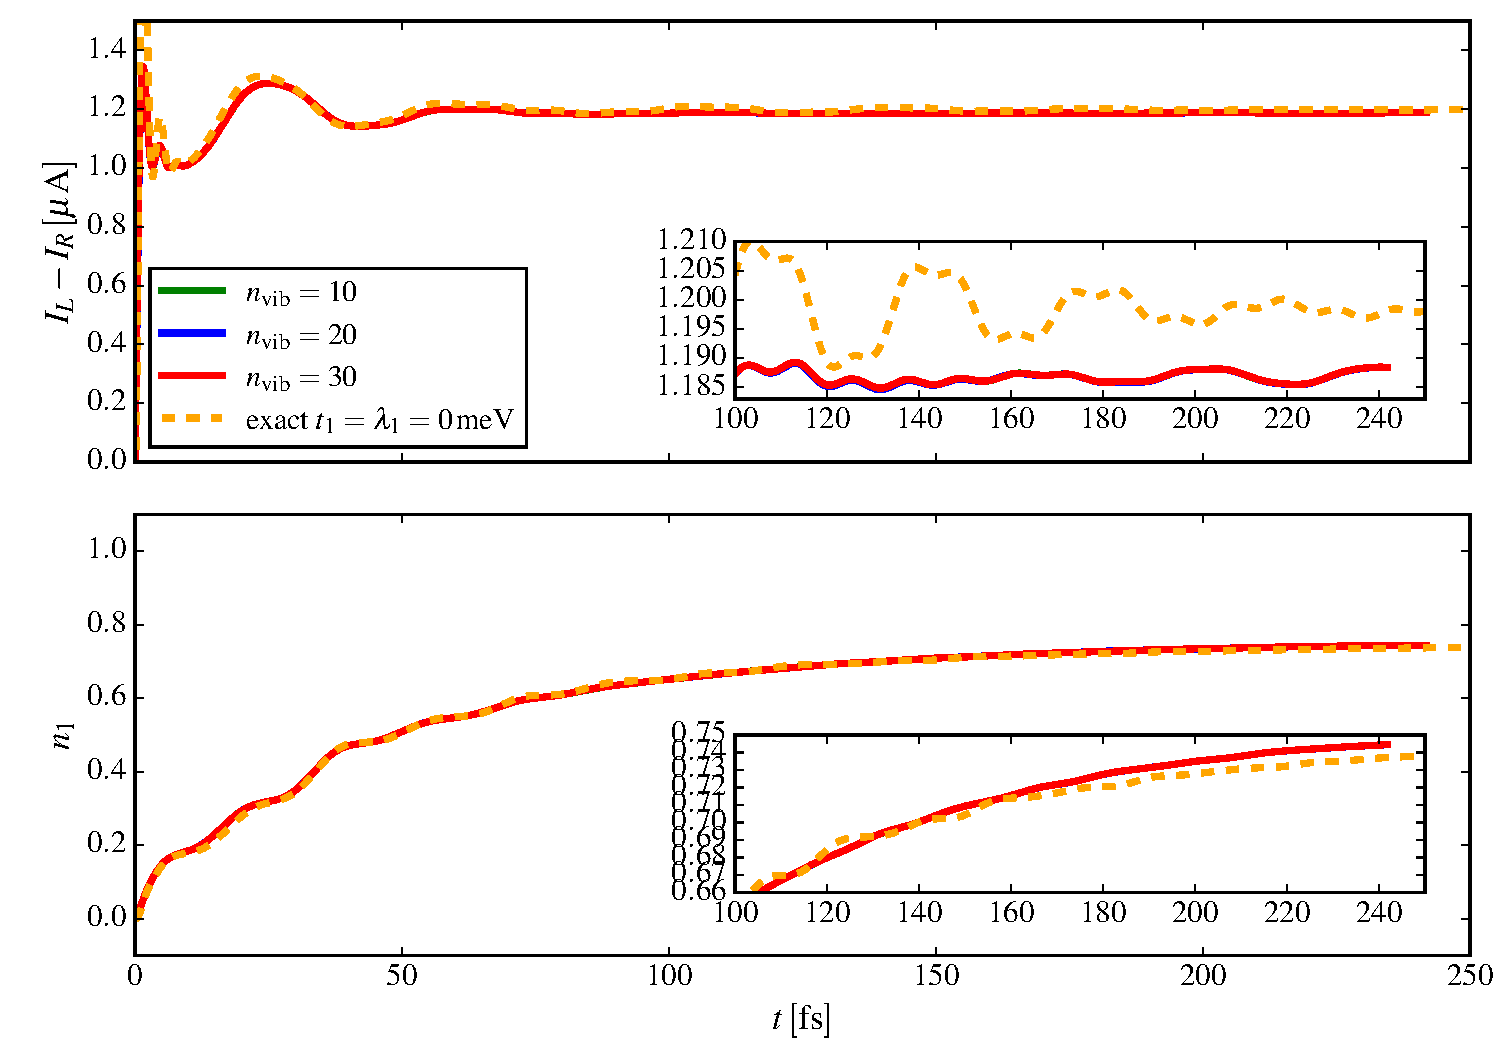
\includegraphics[width=0.85\textwidth]{figs/Comparison_TTHEOM_MFHEOM_Holstein_1x4_noSpin_w0_0.05_V0.48.pdf}
	\caption{Symmetrized current and electronic population on site 1 for $N=4$.}
\end{figure}
\subsection{$N = 8$}
\begin{figure}[!h]
	\centering
	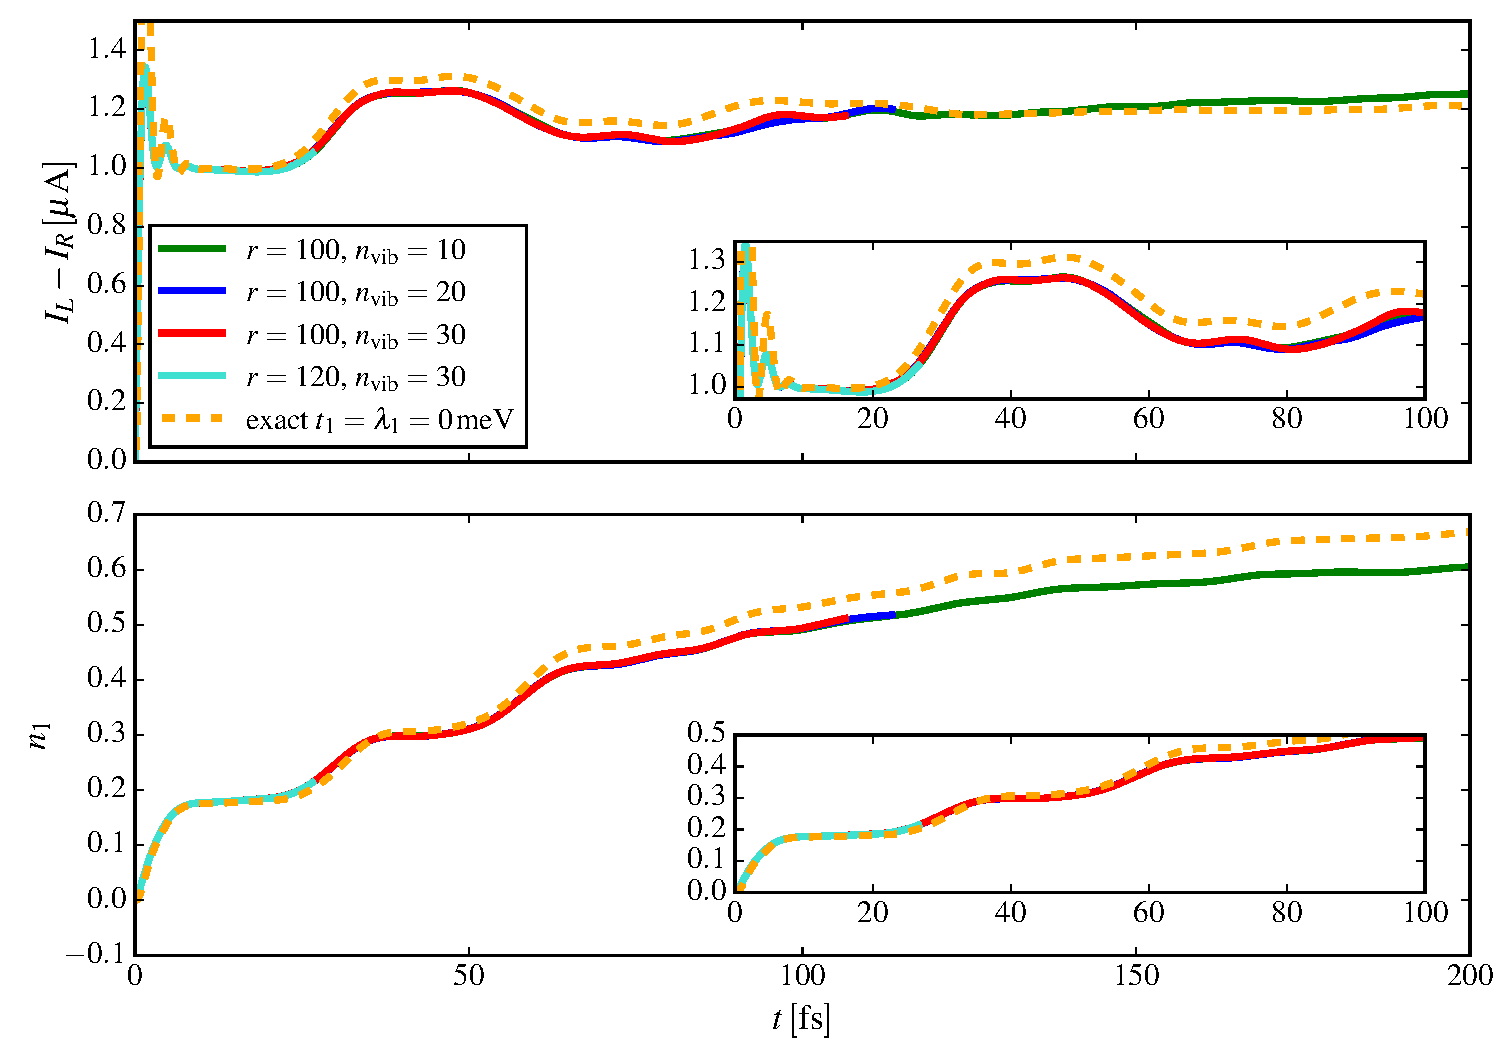
\includegraphics[width=0.85\textwidth]{figs/Comparison_TTHEOM_MFHEOM_Holstein_1x8_noSpin_w0_0.05_V0.48.pdf}
	\caption{Symmetrized current and electronic population on site 1 for $N=8$.}
\end{figure}
\section{Fransson's model}
\subsection{Model}
Fransson considers spinfull electrons in a chain with spin-orbit coupling and a spin-orbit contribution to the electron-phonon coupling
\begin{equation}
	\begin{split}
		\hat{H}_\mathrm{sys} &= \sum_{j,\sigma} \varepsilon_{j\sigma}^\pdagger \hat{d}_{j\sigma}^\dagger \hat{d}_{j\sigma}^\pdagger  +\sum_{j} \omega_{j}^\pdagger \hat{a}_{j}^\dagger \hat{a}_{j}^\pdagger- t_0 \sum_{j\sigma} (\hat{d}_{j\sigma}^\dagger \hat{d}_{j+1,\sigma}^\pdagger + \mathrm{h.c.}) \\&+ \lambda_0^\pdagger\sum_{j\sigma\sigma'} (i\hat{d}_{j\sigma}^\dagger (\vec{v}_j^{(+)}\cdot \bm{\sigma})_{\sigma\sigma'}^\pdagger \hat{d}_{j+2,\sigma'}^\pdagger + \mathrm{h.c.})\\
		&- t_1^\pdagger \sum_{j,\sigma}  \hat{d}_{j\sigma}^\dagger \hat{d}_{j+1\sigma}^\pdagger (\hat{a}_{j}^\dagger + \hat{a}_{j}^\pdagger) \\ & + \lambda_1^\pdagger\sum_{j,\sigma,\sigma'} (i \hat{d}_{j\sigma}^\dagger (\vec{v}_j^{(+)} \cdot \bm{\sigma})_{\sigma\sigma'}^\pdagger \hat{d}_{j+2\sigma'}^\pdagger +\mathrm{h.c.})(\hat{a}_{j}^\dagger + \hat{a}_{j}^\pdagger).
	\end{split}
\end{equation}
The leads are considered to be spin-full, meaning the lead and system-lead hamiltonians are
\begin{align}
	H_\mathrm{leads} &= \sum_{\ell=L,R}\sum_{k\sigma} \varepsilon_{\ell k\sigma}^\pdagger c_{\ell k\sigma}^\dagger  c_{\ell k\sigma}^\pdagger,\\
	H_\mathrm{sys-lead} &= \sum_{\ell k\sigma} (V_{\ell k 1\sigma}^\pdagger c_{\ell k\sigma}^\dagger d_{1\sigma}^\pdagger + V_{\ell k N\sigma}^\pdagger c_{\ell k\sigma}^\dagger d_{N\sigma}^\pdagger + \mathrm{h.c.})
\end{align}
that is only spin-conserving transitions between the leads and the system are allowed. The left lead is ferrimagnetically polarized, which is modeled by a spin-dependent spectral function
\begin{equation}
	\Gamma^{(L)}_1 = \Gamma_0^{(L)} \left(\mathds{1} + P\sigma^z\right)
\end{equation}
with $\Gamma_0^{(\ell)}= \SI{10}{\milli\electronvolt}$ and $P=\frac{1}{2}$.
\clearpage
\subsection{$N=3$}
\begin{figure}[!h]
	\centering
	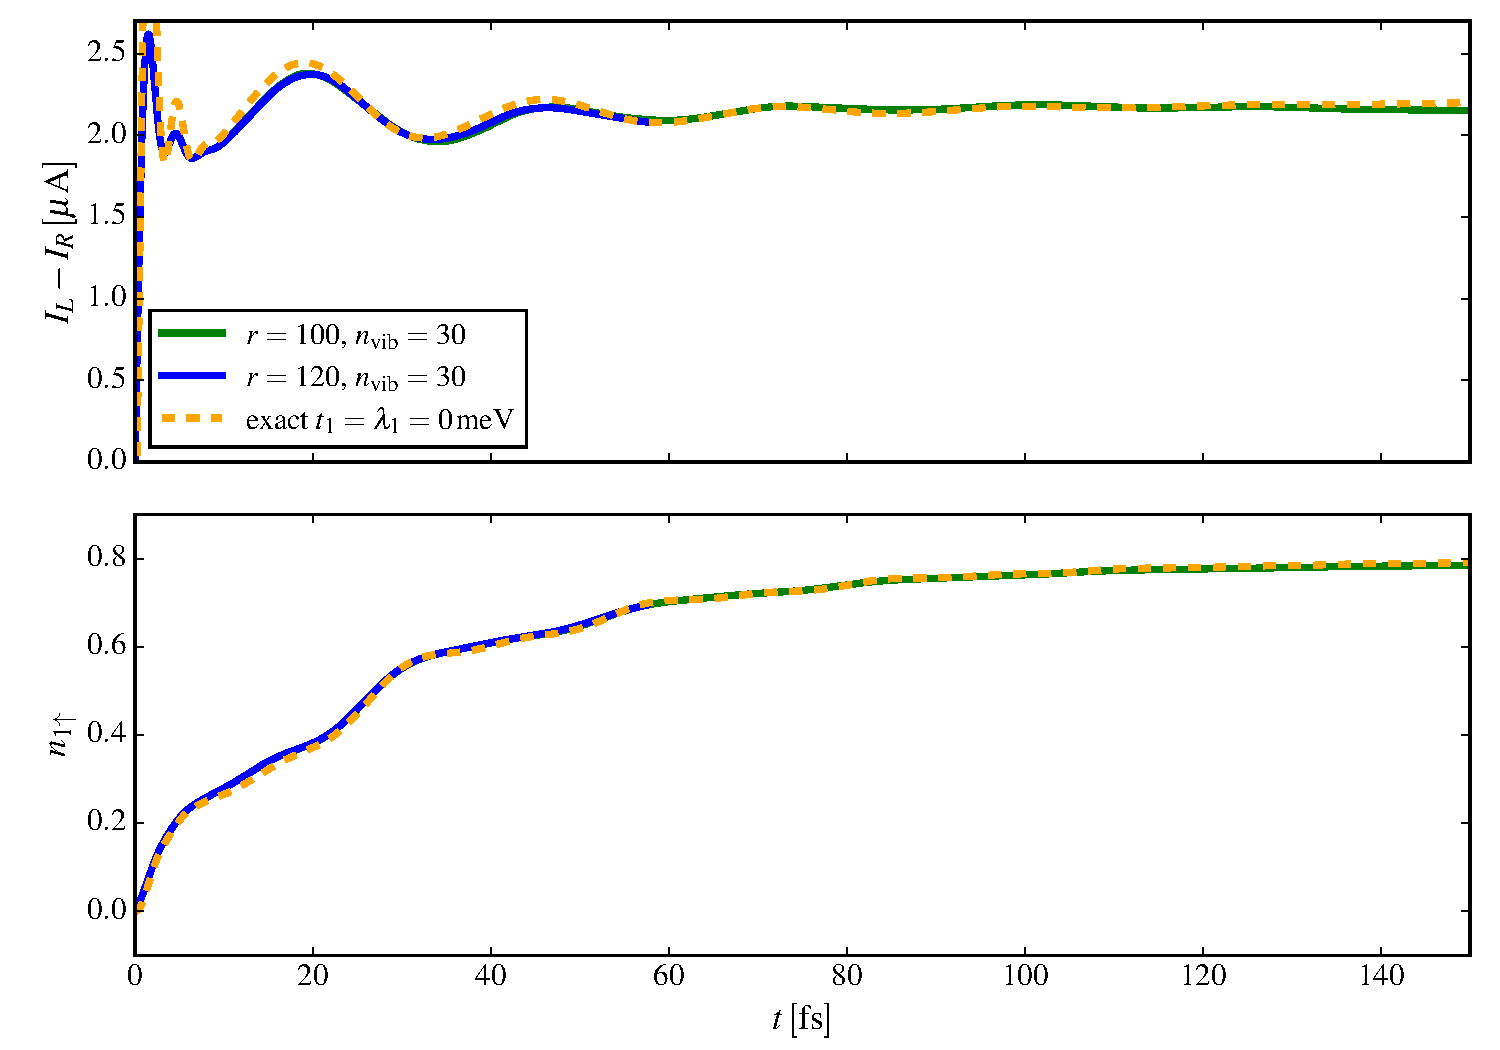
\includegraphics[width=0.85\textwidth]{figs/Comparison_TTHEOM_MFHEOM_Fransson_1x3_w0_0.05_V0.48.pdf}
	\caption{Symmetrized current and electronic population on site 1 in the Fransson model with $N=3$ sites.}
\end{figure}
\subsection{$N=4$}
\begin{figure}[!h]
	\centering
	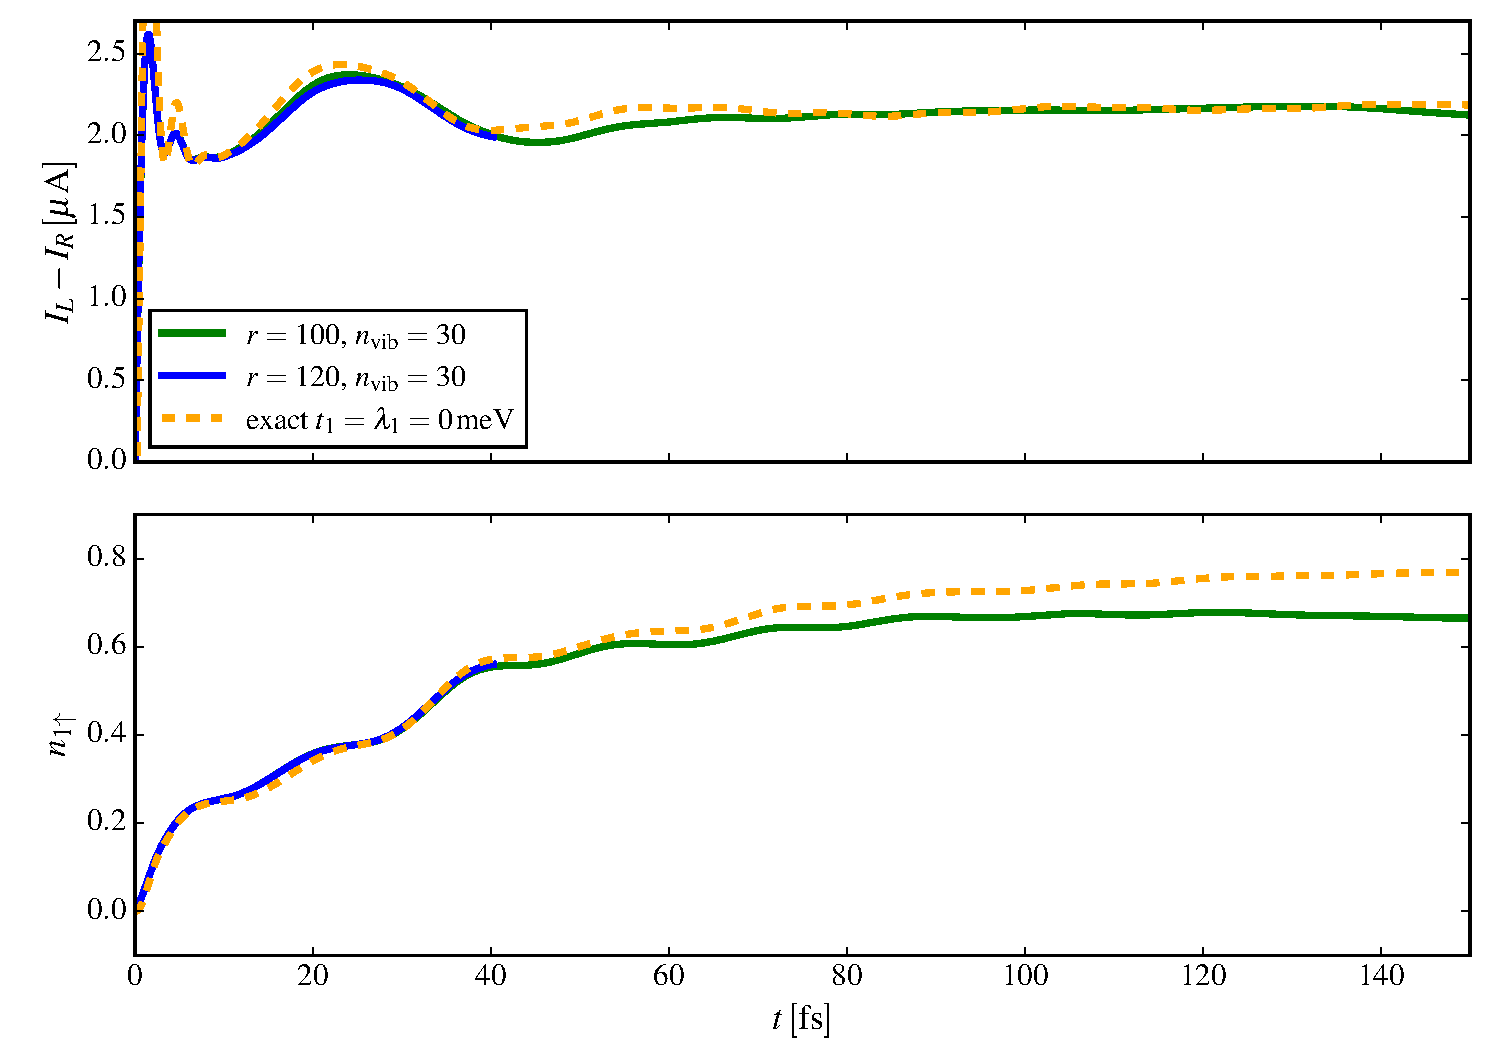
\includegraphics[width=0.85\textwidth]{figs/Comparison_TTHEOM_MFHEOM_Fransson_1x4_w0_0.05_V0.48.pdf}
	\caption{Symmetrized current and electronic population on site 1 in the Fransson model with $N=4$ sites.}
\end{figure}


\section{Holstein model}
%\subsection{Spinless}
\begin{figure}[!h]
	\centering
	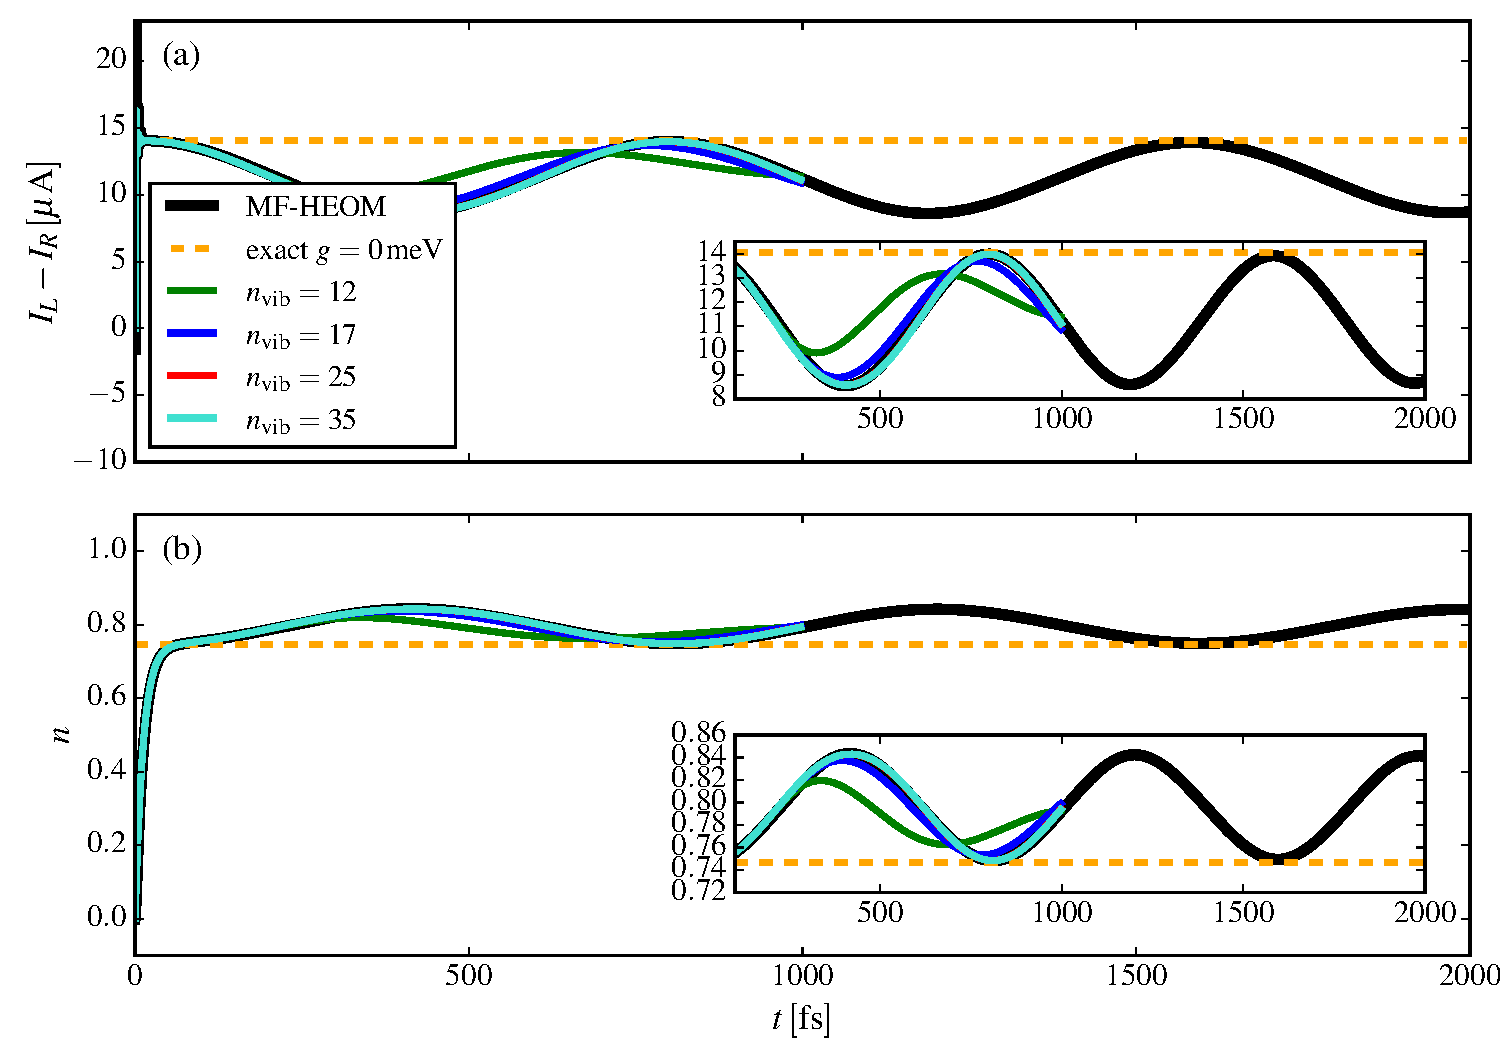
\includegraphics[width=0.85\textwidth]{figs/Comparison_TTHEOM_MFHEOM_Holstein_1x1_noSpin_w0_0.05_V0.48.pdf}
	\caption{Holstein model for $\omega_0=\SI{2}{\milli\electronvolt}$ and $V=\SI{0.48}{\volt}$.}
\end{figure}
%\clearpage
%\subsection{Spinfull}
%\begin{figure}[!h]
%	\centering
%	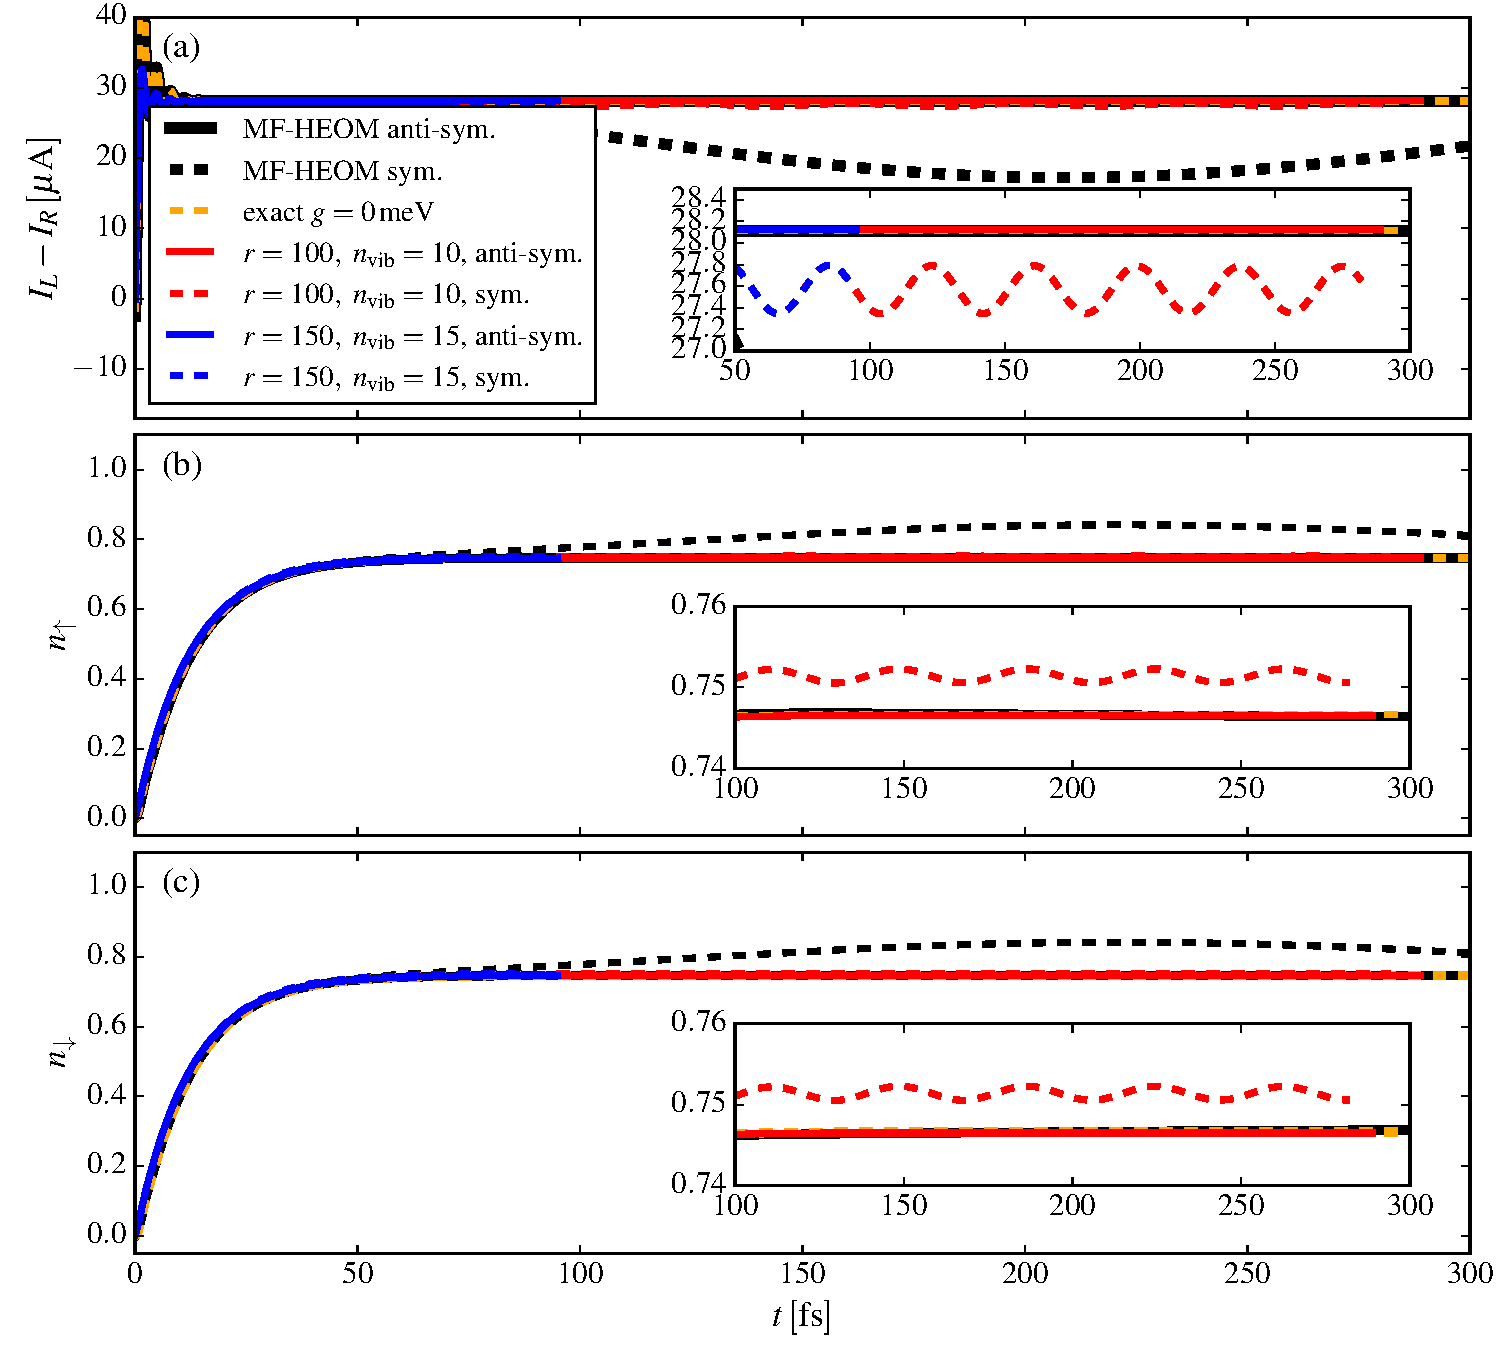
\includegraphics[width=0.9\textwidth]{figs/Comparison_TTHEOM_MFHEOM_Holstein_1x1_Spin_w0_0.05_V0.48.pdf}
%\end{figure}
%\clearpage
\section{Peierls model}

%\subsection{Spinless}
\begin{figure}[!h]
	\centering
	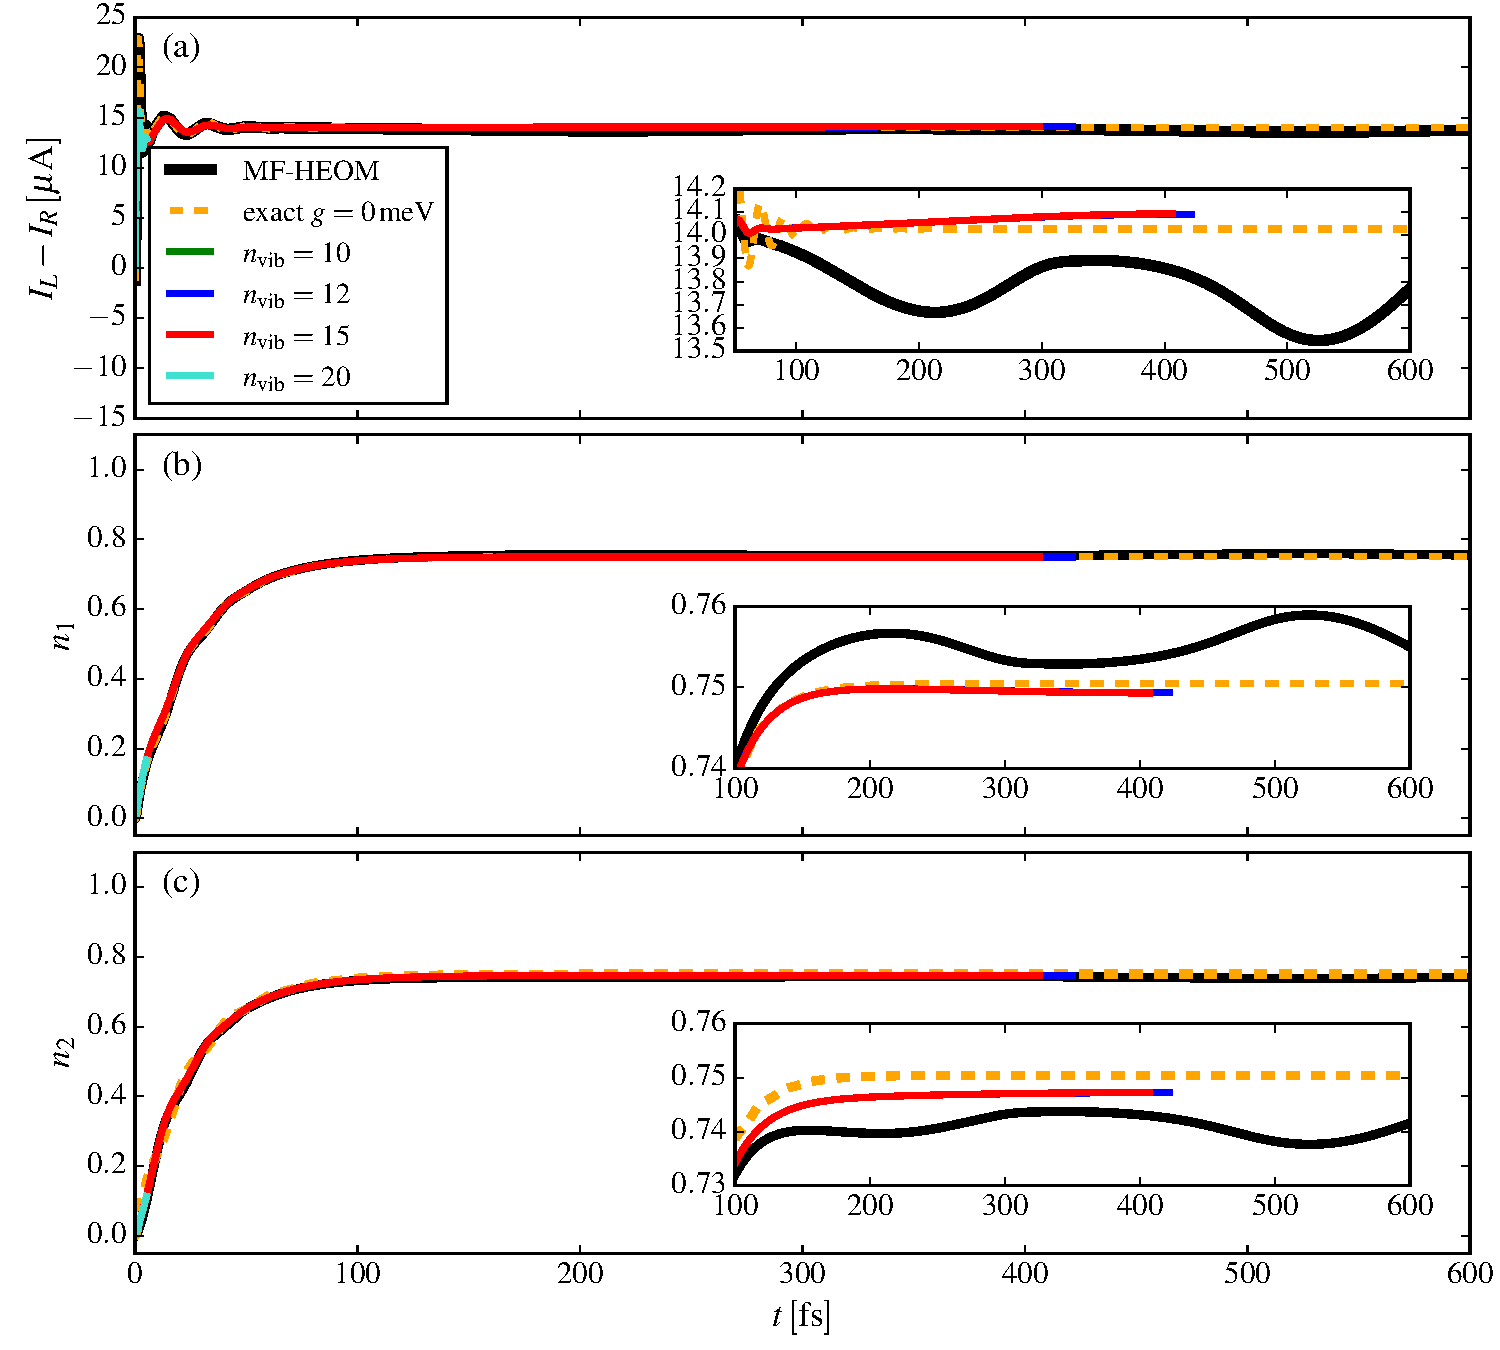
\includegraphics[width=0.85\textwidth]{figs/Comparison_TTHEOM_MFHEOM_Peierls_1x2_noSpin_w0_0.05_V0.48.pdf}
\end{figure}
%\clearpage
%\subsection{Spinfull}
%\begin{figure}[!h]
%	\centering
%	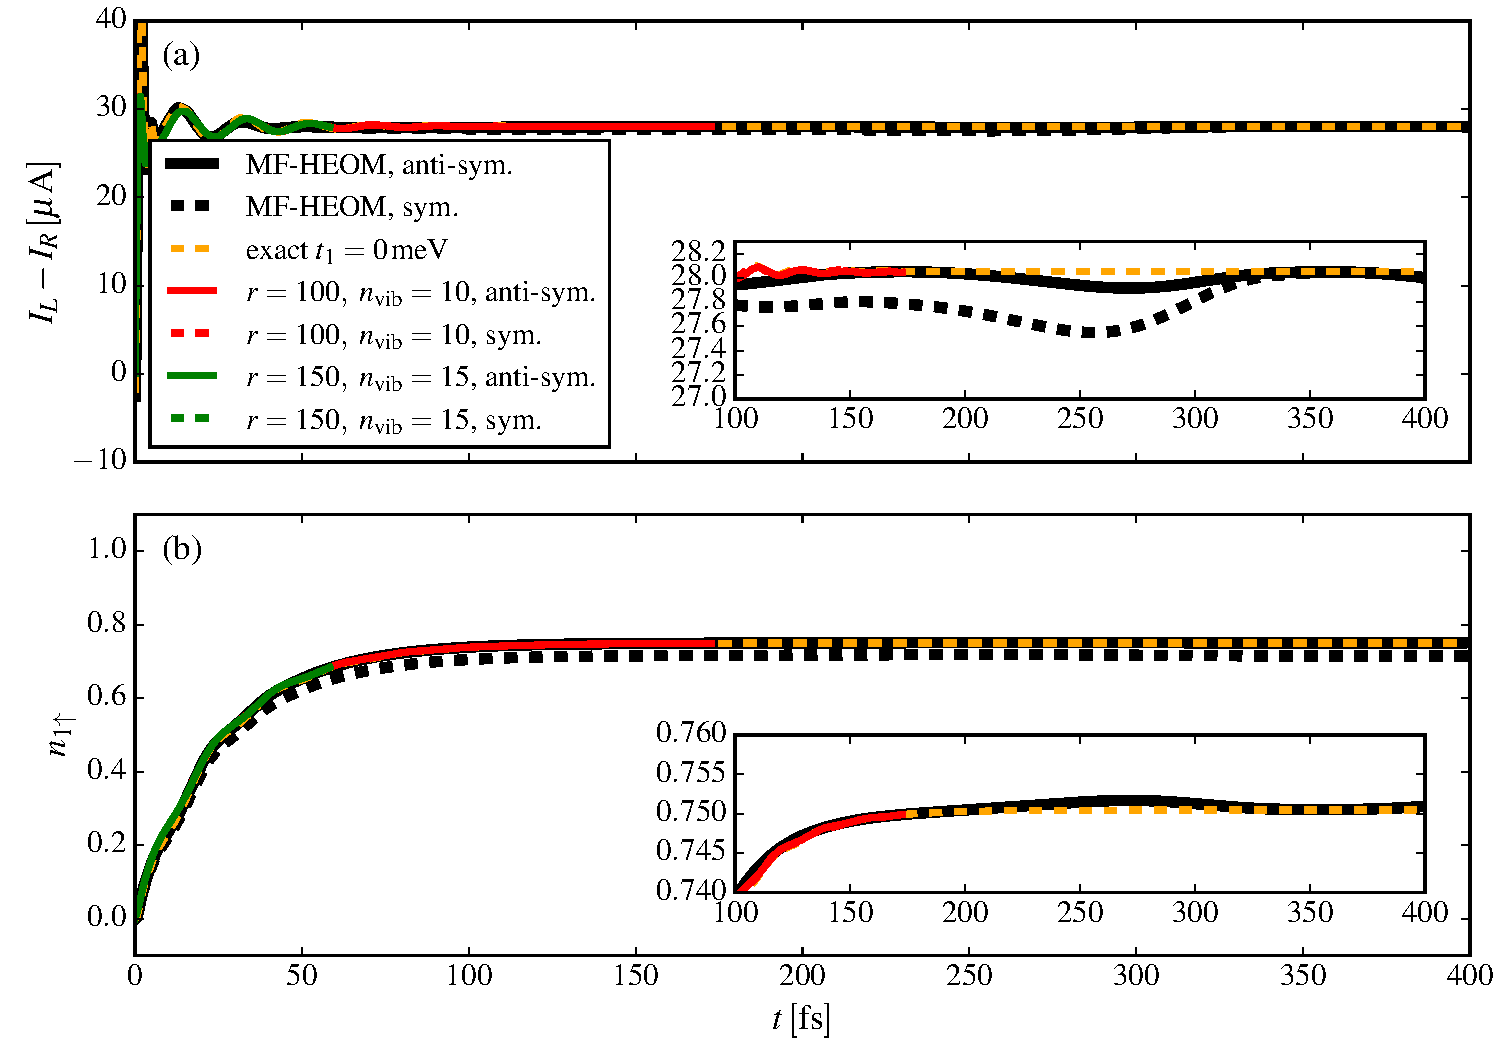
\includegraphics[width=0.9\textwidth]{figs/Comparison_TTHEOM_MFHEOM_Peierls_1x2_Spin_w0_0.05_V0.48.pdf}
%\end{figure}

\end{document}




